\documentclass{article}
\usepackage[utf8]{inputenc}
\usepackage{graphicx}
\usepackage{color}
\usepackage{hyperref}

\PassOptionsToPackage{hyphens}{url}\usepackage{hyperref}
\title{Installation Instruction for Vivado WebPack Edition}
\author{ECN-104 - Digital Logic Design }
\date{Spring 2019}

\hypersetup{
  colorlinks=true,
  allcolors=blue
}

\usepackage{fontspec}

% -----------------------------------------------------------
% Comment the following lines if Adobe Garamond Pro font is
% not available as `AGaramondPro'
\setmainfont{AGaramondPro}[
UprightFont   = *-Regular,
ItalicFont    = *-Italic,
BoldFont      = *-Semibold,
BoldItalicFont= *-BoldItalic
]
% -----------------------------------------------------------

%%%----------%%%----------%%%----------%%%----------%%%
% Command for creating document history items
\newcommand{\histitem}[2]{
  \footnotesize
  \item \textbf{#1}: #2
  \normalsize
}

\begin{document}
\maketitle

For this course we'll be using Xilinx's Vivado, Vivado is one of the
most popular synthesis and HDL design tool. Xilinx provides Vivado
WebPACK edition for free. Follow the instructions given below to
create a new Xilinx account and install Vivado WebPACK edition on your
computer.

\section{Creating a new Xilinx account}
\begin{enumerate}
\item Go to
  \url{https://www.xilinx.com/registration/create-account.html} and
  create a new account.
\end{enumerate}

\section{Downloading the self-extracting installer}
\begin{enumerate}
\item Go to \url{https://www.xilinx.com/support/download.html}.
\item Under the section `\textit{Vivado Design Suite - HLx Editions -
    2018.3 Full Product Installation}', choose the edition depending
  on your operating system.
\item If you are signed in, you will be forwarded to Xilinx's Name and
  Address verification page.
\item Enter your details here and click `\textit{Download}'.
\item If everything goes well, Vivado installer would start getting
  downloaded.
\end{enumerate}

\section{Installing Vivado WebPACK Edition (on Windows)}
\begin{enumerate}
    \item Start the installer, press \textit{Next}
    \item Enter your account details, select \textit{Download and
        Install Now} and press \textit{Next}
    \item Agree to the terms and click \textit{Next}
    \item Choose `\textit{Vivado HL WebPACK}' and press continue
    \item Make sure the checklist on your screen matches
      Fig. \ref{Fig:install_options} and click \textit{Next}.
    \item Choose the installation location and press \textit{Next}
    \item Press \textit{Install}
\end{enumerate}

\begin{figure}[h] \centering 
  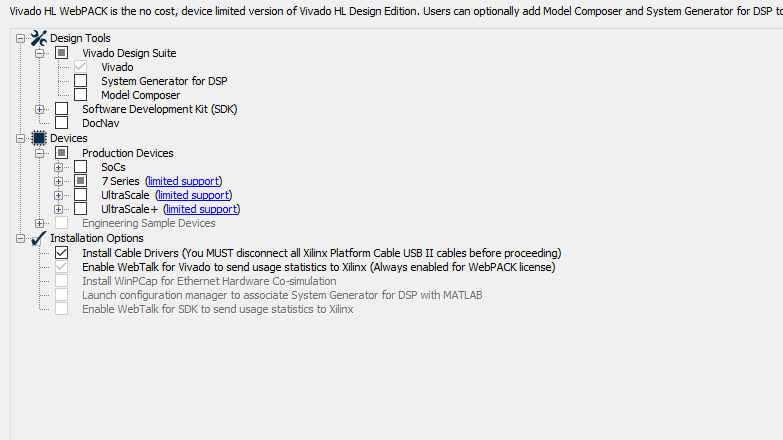
\includegraphics[width=\linewidth]{./images/install_options.png}
  \caption{Components to choose for installation of Vivado.}
  \label{Fig:install_options}
\end{figure}
The installer will now download and install all the required
components.

\section*{Note}
Please ensure that Vivado is functioning before your first tutorial on
Verilog. If anything goes wrong, create a post on Moodle with relevant
details so that we can help you out.

\section*{Common Sources of Error}
\begin{enumerate}
\item Make sure your system date and time are correct. If not, the
  Vivado installer will fail to sign in onto your account.
\item The configuration used in this course requires {$\sim$}16.3 GiB of
  disk space, please ensure you have atleast that much space vacant on
  your installation drive.
\end{enumerate}

\section*{Document History}
\begin{enumerate}
  \histitem{Mon Feb  4 12:33:20 IST 2019}{
    Changes are:
    \begin{enumerate}
    \item Added section \textit{Common Sources of Errors}
    \item Added section \textit{Note}
    \item Add section \textit{Document History}
    \item Updated the tutorial for Vivado 2018.3
    \end{enumerate}
  }
  \histitem{Fri Feb  2 22:52:10 IST 2018}{
    First Edition
  }
\end{enumerate}
\end{document}
